\documentclass{standalone}
\usepackage{tikz}
\usetikzlibrary{patterns, positioning}


\begin{document}
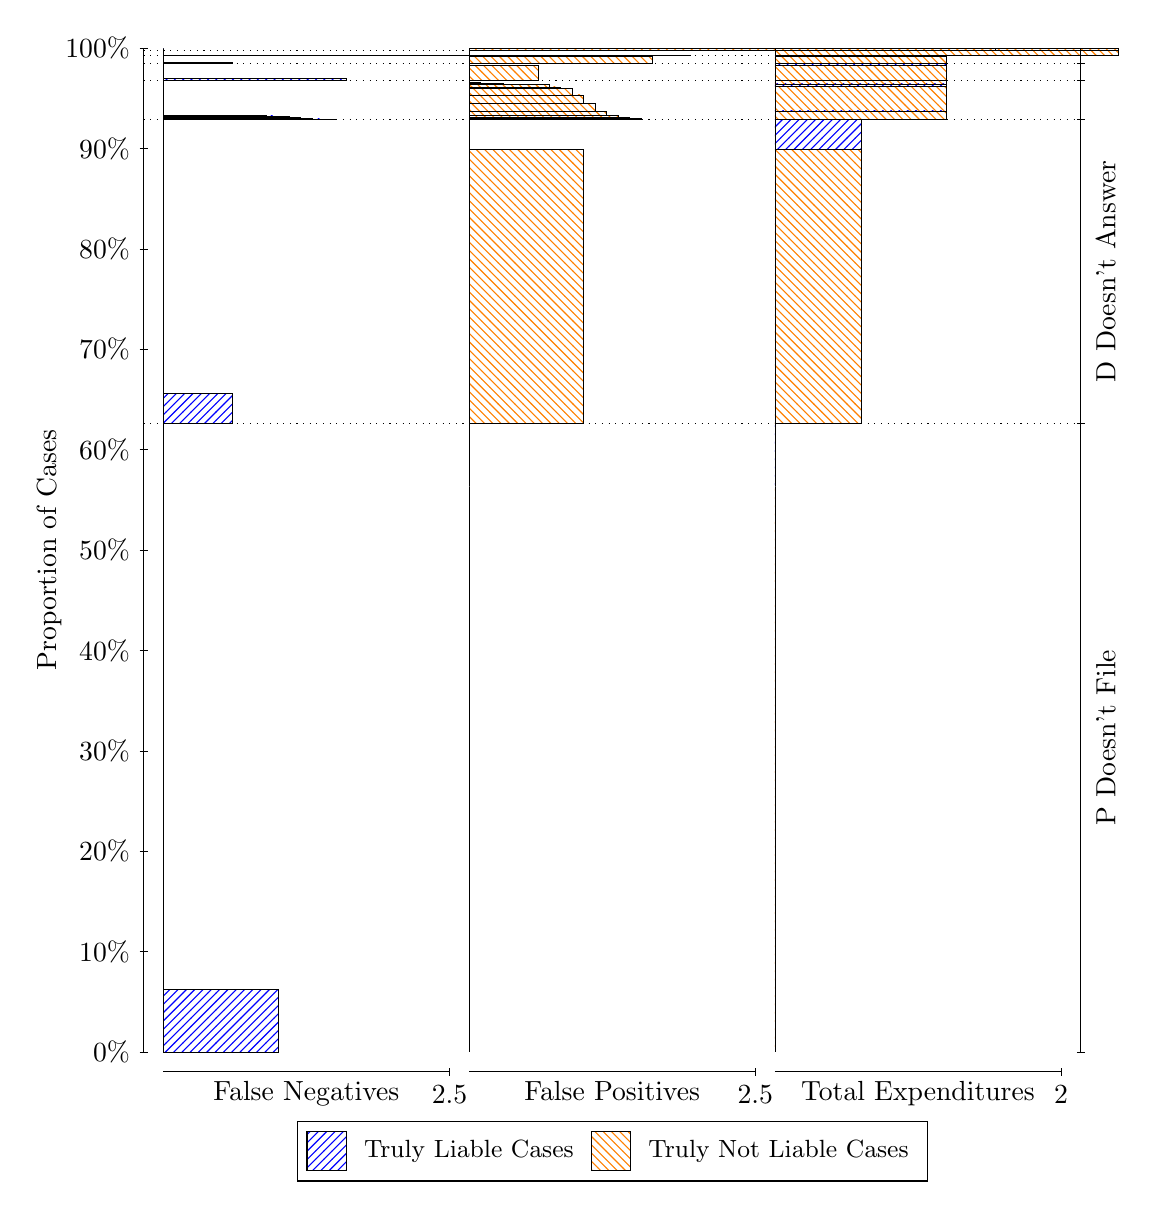
\begin{tikzpicture}
\draw[black, very thin] (1.5,1.75) -- (1.5,14.5);
\node[rotate=90, text=black, anchor=center] at (0.3, 8.125) {Proportion of Cases};
\draw[black, very thin] (1.45,1.75) -- (1.55,1.75);
\node[text=black, anchor=east] at (1.45, 1.75) {0\%};
\draw[black, very thin] (1.45,3.025) -- (1.55,3.025);
\node[text=black, anchor=east] at (1.45, 3.025) {10\%};
\draw[black, very thin] (1.45,4.3) -- (1.55,4.3);
\node[text=black, anchor=east] at (1.45, 4.3) {20\%};
\draw[black, very thin] (1.45,5.575) -- (1.55,5.575);
\node[text=black, anchor=east] at (1.45, 5.575) {30\%};
\draw[black, very thin] (1.45,6.85) -- (1.55,6.85);
\node[text=black, anchor=east] at (1.45, 6.85) {40\%};
\draw[black, very thin] (1.45,8.125) -- (1.55,8.125);
\node[text=black, anchor=east] at (1.45, 8.125) {50\%};
\draw[black, very thin] (1.45,9.4) -- (1.55,9.4);
\node[text=black, anchor=east] at (1.45, 9.4) {60\%};
\draw[black, very thin] (1.45,10.675) -- (1.55,10.675);
\node[text=black, anchor=east] at (1.45, 10.675) {70\%};
\draw[black, very thin] (1.45,11.95) -- (1.55,11.95);
\node[text=black, anchor=east] at (1.45, 11.95) {80\%};
\draw[black, very thin] (1.45,13.225) -- (1.55,13.225);
\node[text=black, anchor=east] at (1.45, 13.225) {90\%};
\draw[black, very thin] (1.45,14.5) -- (1.55,14.5);
\node[text=black, anchor=east] at (1.45, 14.5) {100\%};

\draw[black, very thin] (13.4,1.75) -- (13.4,14.5);
\draw[black, very thin] (13.35,1.75) -- (13.45,1.75);
\node[anchor=west] at (13.35, 1.75) {};
\draw[black, very thin] (13.35,9.7326) -- (13.45,9.7326);
\node[anchor=west] at (13.35, 9.7326) {};
\draw[black, very thin] (13.35,13.593) -- (13.45,13.593);
\node[anchor=west] at (13.35, 13.593) {};
\draw[black, very thin] (13.35,14.092) -- (13.45,14.092);
\node[anchor=west] at (13.35, 14.092) {};
\draw[black, very thin] (13.35,14.303) -- (13.45,14.303);
\node[anchor=west] at (13.35, 14.303) {};
\draw[black, very thin] (13.35,14.402) -- (13.45,14.402);
\node[anchor=west] at (13.35, 14.402) {};
\draw[black, very thin] (13.35,14.474) -- (13.45,14.474);
\node[anchor=west] at (13.35, 14.474) {};
\draw[black, very thin] (13.35,14.5) -- (13.45,14.5);
\node[anchor=west] at (13.35, 14.5) {};

\draw[black, very thin, pattern color=blue, pattern=north east lines] (1.75,1.75) rectangle (3.2033,2.5482);
\draw[black, very thin, pattern color=orange, pattern=north west lines] (1.75,2.5482) rectangle (1.75,9.7326);
\draw[black, very thin, pattern color=blue, pattern=north east lines] (1.75,9.7326) rectangle (2.622,10.117);
\draw[black, very thin, pattern color=orange, pattern=north west lines] (1.75,10.117) rectangle (1.75,13.593);
\draw[black, very thin, pattern color=blue, pattern=north east lines] (1.75,13.593) rectangle (3.93,13.597);
\draw[black, very thin, pattern color=blue, pattern=north east lines] (1.75,13.597) rectangle (3.7847,13.599);
\draw[black, very thin, pattern color=blue, pattern=north east lines] (1.75,13.599) rectangle (3.6393,13.609);
\draw[black, very thin, pattern color=blue, pattern=north east lines] (1.75,13.609) rectangle (3.494,13.621);
\draw[black, very thin, pattern color=blue, pattern=north east lines] (1.75,13.621) rectangle (3.3487,13.633);
\draw[black, very thin, pattern color=blue, pattern=north east lines] (1.75,13.633) rectangle (3.2033,13.639);
\draw[black, very thin, pattern color=blue, pattern=north east lines] (1.75,13.639) rectangle (3.058,13.642);
\draw[black, very thin, pattern color=blue, pattern=north east lines] (1.75,13.642) rectangle (2.9127,13.644);
\draw[black, very thin, pattern color=blue, pattern=north east lines] (1.75,13.644) rectangle (2.7673,13.645);
\draw[black, very thin, pattern color=orange, pattern=north west lines] (1.75,13.645) rectangle (1.75,14.092);
\draw[black, very thin, pattern color=blue, pattern=north east lines] (1.75,14.092) rectangle (4.0753,14.111);
\draw[black, very thin, pattern color=orange, pattern=north west lines] (1.75,14.111) rectangle (1.75,14.303);
\draw[black, very thin, pattern color=blue, pattern=north east lines] (1.75,14.303) rectangle (2.622,14.314);
\draw[black, very thin, pattern color=orange, pattern=north west lines] (1.75,14.314) rectangle (1.75,14.402);
\draw[black, very thin, pattern color=blue, pattern=north east lines] (1.75,14.402) rectangle (8.4353,14.404);
\draw[black, very thin, pattern color=orange, pattern=north west lines] (1.75,14.404) rectangle (1.75,14.474);
\draw[black, very thin, pattern color=orange, pattern=north west lines] (1.75,14.474) rectangle (1.75,14.492);
\draw[black, very thin, pattern color=blue, pattern=north east lines] (1.75,14.492) rectangle (1.75,14.5);
\draw[black, very thin, pattern color=orange, pattern=north west lines] (5.6333,1.75) rectangle (5.6333,8.9344);
\draw[black, very thin, pattern color=blue, pattern=north east lines] (5.6333,8.9344) rectangle (5.6333,9.7326);
\draw[black, very thin, pattern color=orange, pattern=north west lines] (5.6333,9.7326) rectangle (7.0867,13.208);
\draw[black, very thin, pattern color=blue, pattern=north east lines] (5.6333,13.208) rectangle (5.6333,13.593);
\draw[black, very thin, pattern color=orange, pattern=north west lines] (5.6333,13.593) rectangle (7.8133,13.605);
\draw[black, very thin, pattern color=orange, pattern=north west lines] (5.6333,13.605) rectangle (7.668,13.617);
\draw[black, very thin, pattern color=orange, pattern=north west lines] (5.6333,13.617) rectangle (7.5227,13.648);
\draw[black, very thin, pattern color=orange, pattern=north west lines] (5.6333,13.648) rectangle (7.3773,13.7);
\draw[black, very thin, pattern color=orange, pattern=north west lines] (5.6333,13.7) rectangle (7.232,13.799);
\draw[black, very thin, pattern color=orange, pattern=north west lines] (5.6333,13.799) rectangle (7.0867,13.906);
\draw[black, very thin, pattern color=orange, pattern=north west lines] (5.6333,13.906) rectangle (6.9413,13.989);
\draw[black, very thin, pattern color=orange, pattern=north west lines] (5.6333,13.989) rectangle (6.796,14.006);
\draw[black, very thin, pattern color=orange, pattern=north west lines] (5.6333,14.006) rectangle (6.6507,14.04);
\draw[black, very thin, pattern color=blue, pattern=north east lines] (5.6333,14.04) rectangle (6.36,14.041);
\draw[black, very thin, pattern color=blue, pattern=north east lines] (5.6333,14.041) rectangle (6.2147,14.043);
\draw[black, very thin, pattern color=blue, pattern=north east lines] (5.6333,14.043) rectangle (6.0693,14.046);
\draw[black, very thin, pattern color=blue, pattern=north east lines] (5.6333,14.046) rectangle (5.924,14.052);
\draw[black, very thin, pattern color=blue, pattern=north east lines] (5.6333,14.052) rectangle (5.7787,14.064);
\draw[black, very thin, pattern color=blue, pattern=north east lines] (5.6333,14.064) rectangle (5.6333,14.092);
\draw[black, very thin, pattern color=orange, pattern=north west lines] (5.6333,14.092) rectangle (6.5053,14.284);
\draw[black, very thin, pattern color=blue, pattern=north east lines] (5.6333,14.284) rectangle (5.6333,14.303);
\draw[black, very thin, pattern color=orange, pattern=north west lines] (5.6333,14.303) rectangle (7.9587,14.391);
\draw[black, very thin, pattern color=blue, pattern=north east lines] (5.6333,14.391) rectangle (6.5053,14.402);
\draw[black, very thin, pattern color=orange, pattern=north west lines] (5.6333,14.402) rectangle (5.6333,14.472);
\draw[black, very thin, pattern color=blue, pattern=north east lines] (5.6333,14.472) rectangle (5.6333,14.474);
\draw[black, very thin, pattern color=orange, pattern=north west lines] (5.6333,14.474) rectangle (12.319,14.492);
\draw[black, very thin, pattern color=blue, pattern=north east lines] (5.6333,14.492) rectangle (10.865,14.5);
\draw[black, very thin, pattern color=orange, pattern=north west lines] (9.5167,1.75) rectangle (9.5167,8.9344);
\draw[black, very thin, pattern color=blue, pattern=north east lines] (9.5167,8.9344) rectangle (9.5167,9.7326);
\draw[black, very thin, pattern color=orange, pattern=north west lines] (9.5167,9.7326) rectangle (10.607,13.208);
\draw[black, very thin, pattern color=blue, pattern=north east lines] (9.5167,13.208) rectangle (10.607,13.593);
\draw[black, very thin, pattern color=orange, pattern=north west lines] (9.5167,13.593) rectangle (11.697,13.691);
\draw[black, very thin, pattern color=blue, pattern=north east lines] (9.5167,13.691) rectangle (11.697,13.703);
\draw[black, very thin, pattern color=orange, pattern=north west lines] (9.5167,13.703) rectangle (11.697,14.009);
\draw[black, very thin, pattern color=blue, pattern=north east lines] (9.5167,14.009) rectangle (11.697,14.044);
\draw[black, very thin, pattern color=orange, pattern=north west lines] (9.5167,14.044) rectangle (11.697,14.087);
\draw[black, very thin, pattern color=blue, pattern=north east lines] (9.5167,14.087) rectangle (11.697,14.092);
\draw[black, very thin, pattern color=orange, pattern=north west lines] (9.5167,14.092) rectangle (11.697,14.284);
\draw[black, very thin, pattern color=blue, pattern=north east lines] (9.5167,14.284) rectangle (11.697,14.303);
\draw[black, very thin, pattern color=orange, pattern=north west lines] (9.5167,14.303) rectangle (11.697,14.391);
\draw[black, very thin, pattern color=blue, pattern=north east lines] (9.5167,14.391) rectangle (11.697,14.402);
\draw[black, very thin, pattern color=orange, pattern=north west lines] (9.5167,14.402) rectangle (13.877,14.472);
\draw[black, very thin, pattern color=blue, pattern=north east lines] (9.5167,14.472) rectangle (13.877,14.474);
\draw[black, very thin, pattern color=orange, pattern=north west lines] (9.5167,14.474) rectangle (13.877,14.492);
\draw[black, very thin, pattern color=blue, pattern=north east lines] (9.5167,14.492) rectangle (13.877,14.5);
\draw[black, dotted] (1.5,9.7326) -- (13.4,9.7326);
\draw[black, dotted] (1.5,13.593) -- (13.4,13.593);
\draw[black, dotted] (1.5,14.092) -- (13.4,14.092);
\draw[black, dotted] (1.5,14.303) -- (13.4,14.303);
\draw[black, dotted] (1.5,14.402) -- (13.4,14.402);
\draw[black, dotted] (1.5,14.474) -- (13.4,14.474);
\draw[black, very thin] (1.75,1.5) -- (5.3833,1.5);
\node[text=black, anchor=north] at (3.5667, 1.5) {False Negatives};
\draw[black, very thin] (5.3833,1.45) -- (5.3833,1.55);
\node[text=black, anchor=north] at (5.3833, 1.45) {2.5};

\draw[black, very thin] (5.6333,1.5) -- (9.2667,1.5);
\node[text=black, anchor=north] at (7.45, 1.5) {False Positives};
\draw[black, very thin] (9.2667,1.45) -- (9.2667,1.55);
\node[text=black, anchor=north] at (9.2667, 1.45) {2.5};

\draw[black, very thin] (9.5167,1.5) -- (13.15,1.5);
\node[text=black, anchor=north] at (11.333, 1.5) {Total Expenditures};
\draw[black, very thin] (13.15,1.45) -- (13.15,1.55);
\node[text=black, anchor=north] at (13.15, 1.45) {2};

\node[text=black, centered, rotate=90] at (13.72, 5.7413) {P Doesn't File};
\node[text=black, centered, rotate=90] at (13.72, 11.663) {D Doesn't Answer};






\draw (7.449999999999999,1.5) node[draw=none] (baseCoordinate) {};
\begin{scope}[align=center]
        \matrix[scale=0.5, draw=black, below=0.5cm of baseCoordinate, nodes={draw}, column sep=0.1cm]{
            \node[rectangle, draw, minimum width=0.5cm, minimum height=0.5cm, pattern color=blue, pattern=north east lines] {}; &
            \node[draw=none, font=\small, text=black] (B) {Truly Liable Cases}; &
            \node[rectangle, draw, minimum width=0.5cm, minimum height=0.5cm, pattern color=orange, pattern=north west lines] {}; &
            \node[draw=none, font=\small, text=black] (B) {Truly Not Liable Cases}; \\
            };
\end{scope}

\end{tikzpicture}
\end{document}